% CH6 reading draft, 8 September 2026.
% Structure follows Chapters/CH6_object_definition.tex.
% Analysis blueprint: ANA_EXOT_2025_06_INT1, 20 April 2026, Section 5.
% Paper cross-check: arXiv:2606.02067v1, Sections 5 and 7.
% Source decisions and unresolved production details: CH6_source_notes.md.
\chapter{Object Reconstruction and Identification}
\label{chapter:object_reconstruction}

Hadronically decaying $\tau$-leptons, electrons, muons and jets are used in this analysis.
This chapter describes their reconstruction, identification and calibration, followed by overlap removal and the reconstruction of $\met$.

These objects are reconstructed and identified using detector measurements.
Tracks are used to determine charged-particle momenta and production vertices, while energy deposits are measured in the calorimeters.
The reconstructed energies and momenta are calibrated to correct biases in the detector response.
Simulated event weights are further corrected using efficiency scale factors.


\section{Tracks}
\label{sec:ch6_tracks}

\subsection{Reconstruction}

A track is reconstructed by fitting the trajectory of a charged particle to measurements in the ID.
Its momentum and charge are determined from the curvature in the magnetic field, while its position near the beam line is used to associate it with a production vertex.
Track reconstruction is performed in the following stages~\cite{ATLAS2017DenseTracking}:
\begin{enumerate}
    \item \textbf{Space-point formation.} Signals in neighbouring channels of a silicon sensor are grouped into clusters. Three-dimensional space points are obtained from pixel clusters or from paired measurements on the two sides of an SCT module.
    \item \textbf{Seeding and track finding.} Combinations of space points are used to form track seeds. These seeds are extended through the silicon layers with a combinatorial Kalman filter, in which the trajectory and its uncertainty are updated as compatible measurements are added. Multiple scattering and energy loss in the detector material are included in the fit.
    \item \textbf{Ambiguity resolution.} Candidates are ranked using their fit quality, assigned clusters and missing expected measurements. Duplicate or incompatible candidates are rejected, while shared clusters are treated to retain nearby physical tracks where possible.
    \item \textbf{TRT extension.} Accepted silicon tracks are extrapolated into the TRT, and compatible measurements are included in a further fit.
\end{enumerate}

\subsection{Track parameters and quality}

The fitted trajectory is specified by five parameters at its point of closest approach to a reference beam line:
\begin{itemize}
    \item $d_0$ and $z_0$: the signed transverse impact parameter and the longitudinal coordinate at closest approach.
    \item $\phi_0$ and $\theta$: the azimuthal and polar angles of the momentum.
    \item $q/p$: the electric charge divided by the momentum magnitude.
\end{itemize}
Their uncertainties and correlations are described by the covariance matrix of the fit.
The transverse impact-parameter significance, $d_0/\sigma(d_0)$, measures the displacement in units of its uncertainty.
For association with a vertex at $z_{\mathrm{PV}}$, the longitudinal separation is expressed as
\begin{align}
    \Delta z_0\sin\theta=(z_0-z_{\mathrm{PV}})\sin\theta.
    \label{eq:ch6_track_longitudinal}
\end{align}

Track-quality requirements are imposed on the hit content, fit quality and number of missing expected hits.
Additional requirements depend on how the tracks are used: prompt-lepton tracks are required to be compatible with the primary vertex, whereas displaced tracks are retained for heavy-flavour tagging.
The corresponding selections are specified below for each reconstructed object.

\section{Primary vertex}
\label{sec:ch6_primary_vertex}

\subsection{Reconstruction}

Collision vertices are reconstructed from tracks compatible with a common origin~\cite{ATLAS2015Vertex}.
Candidate positions are first identified from the longitudinal distribution of tracks near the beam line.
The vertex positions are then fitted using the track parameters and their uncertainties, with reduced weights assigned to incompatible tracks.
Tracks that are not assigned to a fitted vertex are considered when searching for further vertices.
Several collision vertices can therefore be reconstructed in an event containing pile-up.

\subsection{Primary-vertex selection}

The primary vertex associated with the hard scattering is selected from vertices with at least two tracks satisfying $\pT>500~\MeV$~\cite{ATLAS2026LQTauNu}.
The vertex with the largest sum of squared track transverse momenta is chosen:
\begin{align}
    v_{\mathrm{PV}}=\operatorname*{arg\,max}_{v}
    \sum_{i\in v}p_{\mathrm{T},i}^{\,2}.
    \label{eq:ch6_primary_vertex}
\end{align}
Energetic tracks are given greater weight by this criterion, favouring the hard scattering over additional soft collisions.
Events without a qualifying vertex are rejected.
The selected vertex is used as the reference for prompt-lepton selection, isolation, pile-up jet rejection and the track contribution to $\met$.

\section{Electrons}
\label{sec:ch6_electrons}

\subsection{Reconstruction}

An electron is reconstructed from an ID track matched to an electromagnetic shower in the calorimeter.
Bremsstrahlung photons emitted in the upstream material can spread the shower energy over several clusters and alter the curvature of the electron track.
Both effects are treated in the reconstruction~\cite{ATLAS2019ElectronPerformance}:
\begin{enumerate}
    \item \textbf{Calorimeter clustering.} Neighbouring cells are grouped into topological clusters according to their signal significance above the expected noise. Clusters with a substantial electromagnetic energy fraction are used as electron seeds.
    \item \textbf{Track refitting and matching.} Electron-track candidates are refitted with a Gaussian-sum filter, in which a mixture of Gaussian components is used to describe radiative energy losses. The refitted tracks are extrapolated to the calorimeter and matched to the clusters.
    \item \textbf{Supercluster formation.} Nearby clusters are added to the seed to recover energy from bremsstrahlung. Additional clusters sharing the matched electron track can be collected over a wider region in $\phi$. The resulting variable-size supercluster is matched to the electron track to form the candidate.
\end{enumerate}
The cluster association is illustrated in Figure~\ref{fig:ch6_electron_supercluster}.
The wider collection in $\phi$ helps recover energy separated from the electron by its bending in the magnetic field.

\begin{figure}[htbp]
    \centering
    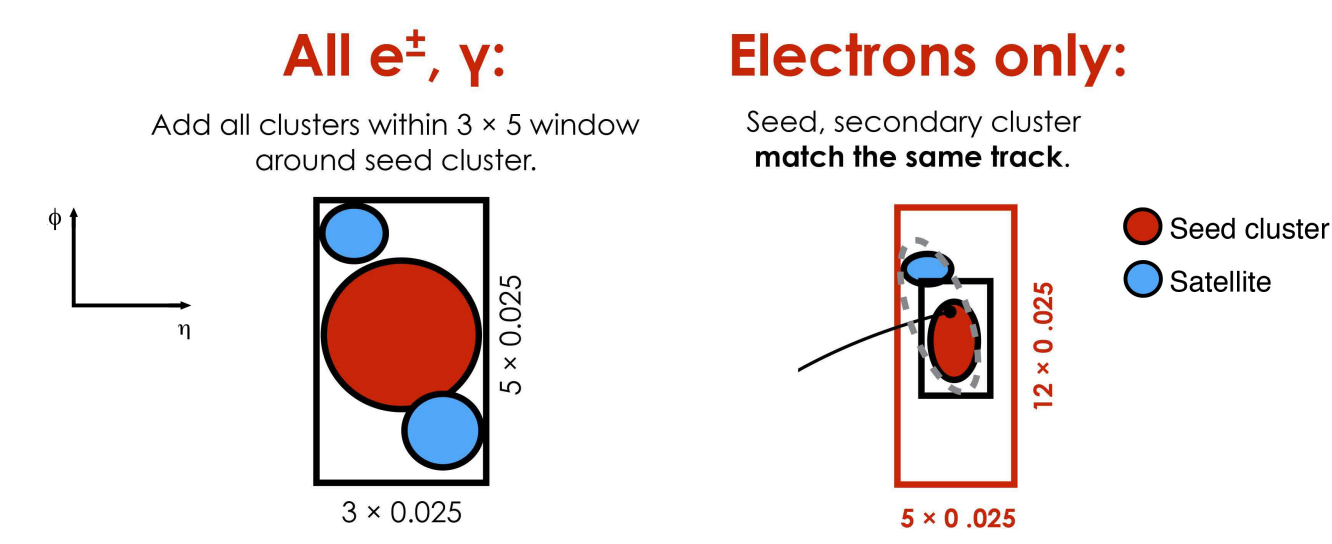
\includegraphics[width=0.75\textwidth]{output/ch6/figures/electron_superclusters.png}
    \caption{Cluster association for electron superclusters. Seed and additional clusters are shown in red and blue, respectively. Geometrically nearby clusters are collected, and a wider association is allowed for clusters sharing the electron track. The electron-relevant part of the supercluster diagram is reproduced from Ref.~\cite{ATLAS2019ElectronPerformance}.}
    \label{fig:ch6_electron_supercluster}
\end{figure}

\subsection{Identification}

Electron candidates are distinguished from hadronic showers and converted photons using a likelihood discriminant~\cite{ATLAS2019ElectronReco}.
Its inputs describe the shower shapes and hadronic leakage, the track hit content, and the agreement between the track and calorimeter measurements.
The \texttt{Loose}, \texttt{Medium} and \texttt{Tight} working points provide increasing background rejection at the cost of electron efficiency.

Baseline electrons are the initial candidates used for object counting and overlap removal.
The following requirements are imposed:
\begin{itemize}
    \item $\pT>10~\GeV$ and $|\eta|<2.47$, excluding $1.37<|\eta|<1.52$.
    \item \texttt{TightLH} identification and a calorimeter cluster passing the object-quality requirements.
    \item $|d_0|/\sigma(d_0)<5$ and $|\Delta z_0\sin\theta|<0.5~\mm$.
\end{itemize}
The impact-parameter requirements suppress electrons from displaced decays and tracks incompatible with the primary vertex.
Clusters in regions with known calorimeter defects are rejected, including the affected end-cap high-voltage regions in the 2016 data.

\subsection{Isolation}

Prompt electrons are separated from electrons inside hadronic jets by requiring little additional activity around the candidate.
Two isolation quantities are used~\cite{ATLAS2019ElectronPerformance}:
\begin{itemize}
    \item \textbf{Track isolation}: the scalar sum of the transverse momenta of nearby tracks associated with the primary vertex, excluding the electron track. The cone radius is reduced at high electron $\pT$ to limit contamination from nearby activity.
    \item \textbf{Calorimeter isolation}: the transverse energy around the electron after subtracting its own shower contribution and correcting for pile-up and shower leakage.
\end{itemize}
Baseline electrons are required to pass \texttt{Loose\_VarRad} isolation.
Signal electrons used in the analysis regions additionally pass \texttt{HighPtCaloOnly} isolation to suppress high-$\pT$ backgrounds.
Their momentum thresholds are specified with the region definitions in Chapter~\ref{chapter:event_selection}.

\subsection{Calibration}

The electron energy is calibrated for losses in upstream material, energy outside the cluster and variations in detector response~\cite{ATLAS2019ElectronPerformance}.
The residual energy scale is constrained using the reconstructed mass in $\zee$ events, and the simulated resolution is adjusted to describe the data.
Reconstruction, identification and isolation efficiencies are measured with the tag-and-probe method: one well-identified electron selects a resonance decay, and the second electron is used to test the requirement under study after background subtraction.
For a selection efficiency $\epsilon$, the scale factor is defined as
\begin{align}
    \mathrm{SF}=\frac{\epsilon_{\mathrm{data}}}{\epsilon_{\mathrm{MC}}}.
    \label{eq:ch6_efficiency_sf}
\end{align}
The appropriate scale factors are applied to simulated event weights for the electron working points used in the analysis.

\section{Muons}
\label{sec:ch6_muons}

\subsection{Reconstruction}

Muons are reconstructed using tracks in the ID and MS, together with their energy deposits in the calorimeters~\cite{ATLAS2021MuonID}.
Their relatively small energy loss allows most muons to reach the MS.
The main reconstruction categories are:
\begin{itemize}
    \item \textbf{Combined muons}: ID and MS tracks are matched and fitted together, including the energy loss between the two tracking systems.
    \item \textbf{Segment-tagged muons}: an ID track is matched to one or more local track segments in the MS when a complete MS track is unavailable.
    \item \textbf{Calorimeter-tagged muons}: an ID track is matched to calorimeter deposits compatible with a minimum-ionising particle. Acceptance is recovered in regions with limited MS coverage.
    \item \textbf{MS-extrapolated muons}: an MS track is extrapolated towards the interaction region without a matched ID track. This category extends reconstruction beyond the ID acceptance and is not used by the $|\eta|<2.5$ selection here.
\end{itemize}

\subsection{Identification}

Muon identification is based on the detector hit content, fit quality and consistency of the independent ID and MS momentum measurements~\cite{ATLAS2021MuonID}.
These requirements suppress hadrons decaying in flight and incorrectly matched tracks.
Baseline muons are required to satisfy:
\begin{itemize}
    \item $\pT>10~\GeV$ and $|\eta|<2.5$.
    \item \texttt{Loose} identification.
    \item $|d_0|/\sigma(d_0)<3$ and $|\Delta z_0\sin\theta|<0.5~\mm$.
\end{itemize}
Additional reconstruction categories are retained by the \texttt{Loose} working point to improve efficiency.
Signal muons are required to pass \texttt{Medium} identification, with more restrictive requirements on the reconstruction quality.

\subsection{Isolation}

Muons from heavy-flavour decays are often accompanied by other particles inside a jet.
They are suppressed using track and calorimeter isolation, defined by the surrounding activity after excluding the muon's own contribution~\cite{ATLAS2021MuonID}.
The track cone is reduced as the muon $\pT$ increases.
The \texttt{Loose\_VarRad} working point is applied to baseline muons, while \texttt{Tight\_VarRad} is additionally required for signal muons.

\subsection{Calibration}

The muon momentum scale and resolution are calibrated using resonance decays, particularly $\zmumu$ and $J/\psi\rightarrow\mu\mu$~\cite{ATLAS2023MuonCalibration}.
The reconstructed mass distributions constrain biases from the magnetic-field description, detector alignment and material modelling.
The corrections are applied to the combined momentum measurement used in the analysis.
Reconstruction, identification and isolation scale factors are measured with tag-and-probe samples and applied to simulated event weights for the selected working points~\cite{ATLAS2021MuonID}.

\input{output/ch6/sections/05_hadronic_taus}
\input{output/ch6/sections/06_jets}
\input{output/ch6/sections/07_flavour_tagging}
\section{Overlap removal}
\label{sec:ch6_overlap}

\subsection{Shared signals and matching}

The same detector activity can be reconstructed as more than one object.
For example, an electron shower can also form a jet, while a hadronic tau candidate is seeded by a calorimeter jet.
An ordered overlap-removal procedure is applied to the baseline candidates to resolve these ambiguities before event selection.
Only objects surviving an earlier step are considered in subsequent steps.

Geometrical overlaps are evaluated with the rapidity distance $\Delta R_y$ defined in Eq.~\eqref{eq:ch6_rapidity}.
Shared ID tracks are also used to identify duplicate electron and muon interpretations.
For muon--jet matching, \emph{ghost association} is used: an object with negligible momentum is placed along the muon direction during jet clustering, and the jet containing it is identified.
The association is therefore determined by the clustering without changing the jet momentum.

\subsection{Removal sequence}

The following steps are applied in order:
\begin{enumerate}
    \item \textbf{Electron--electron}: when two electrons share an ID track, the electron with lower $\pT$ is removed.
    \item \textbf{Tau--electron}: a tau candidate within $\Delta R_y<0.2$ of an electron is removed.
    \item \textbf{Tau--muon}: a tau candidate within $\Delta R_y<0.2$ of a muon is removed.
    \item \textbf{Calorimeter-tagged muon--electron}: a calorimeter-tagged muon sharing the electron ID track is removed.
    \item \textbf{Electron--muon}: an electron sharing an ID track with a remaining muon is removed.
    \item \textbf{Jet--electron}: a jet within $\Delta R_y<0.2$ of an electron is removed.
    \item \textbf{Electron--jet}: an electron within $\Delta R_y<0.4$ of a remaining jet is removed.
    \item \textbf{Jet--muon}: a jet with fewer than three associated tracks is removed if the muon is ghost-associated with it.
    \item \textbf{Muon--jet}: a muon within $\Delta R_y<0.4$ of a remaining jet is removed.
    \item \textbf{Jet--tau}: a jet within $\Delta R_y<0.2$ of a remaining tau candidate is removed.
\end{enumerate}

The inner electron--jet step retains the electron interpretation of an electromagnetic shower, whereas the outer step rejects electrons embedded in surviving hadronic jets.
For muon--jet overlaps, the small track multiplicity is used to recognise a jet candidate dominated by activity associated with the muon.
The last step retains the tau interpretation of an overlapping jet.
The separate low-$\pT$ muon rejection in tau identification, described in Section~\ref{sec:ch6_tau}, is applied in addition to this baseline-object sequence.

\input{output/ch6/sections/09_missing_momentum}
